\documentclass[a4paper,12pt]{article}

%%% Работа с русским языком
\usepackage{cmap}					% поиск в PDF
\usepackage{mathtext} 				% русские буквы в формулах
\usepackage[T2A]{fontenc}			% кодировка
\usepackage[utf8]{inputenc}			% кодировка исходного текста
\usepackage[english,russian]{babel}	% локализация и переносы
\usepackage{xcolor}
\usepackage{hyperref}
 % Цвета для гиперссылок
\definecolor{linkcolor}{HTML}{799B03} % цвет ссылок
\definecolor{urlcolor}{HTML}{799B03} % цвет гиперссылок

\hypersetup{pdfstartview=FitH,  linkcolor=linkcolor,urlcolor=urlcolor, colorlinks=true}

%%% Дополнительная работа с математикой
\usepackage{amsfonts,amssymb,amsthm,mathtools} % AMS
\usepackage{amsmath}
\usepackage{icomma} % "Умная" запятая: $0,2$ --- число, $0, 2$ --- перечисление

%% Номера формул
%\mathtoolsset{showonlyrefs=true} % Показывать номера только у тех формул, на которые есть \eqref{} в тексте.

%% Шрифты
\usepackage{euscript}	 % Шрифт Евклид
\usepackage{mathrsfs} % Красивый матшрифт

%% Свои команды
\DeclareMathOperator{\sgn}{\mathop{sgn}}

%% Перенос знаков в формулах (по Львовскому)
\newcommand*{\hm}[1]{#1\nobreak\discretionary{}
{\hbox{$\mathsurround=0pt #1$}}{}}
% графика
\usepackage{graphicx}
\graphicspath{{pictures/}}
\DeclareGraphicsExtensions{.pdf,.png,.jpg}
\author{Бурмашев Григорий, БПМИ-208}
\title{Матан, дз -- 7}
\date{\today}
\begin{document}
\maketitle
\section*{Номер 1}
Хотим выразить формулу для:
 \begin{equation*}
\begin{gathered}
\mu(A \cap  B \cap  C)
\end{gathered}
\end{equation*}
Из конспекта знаем:
\begin{center}
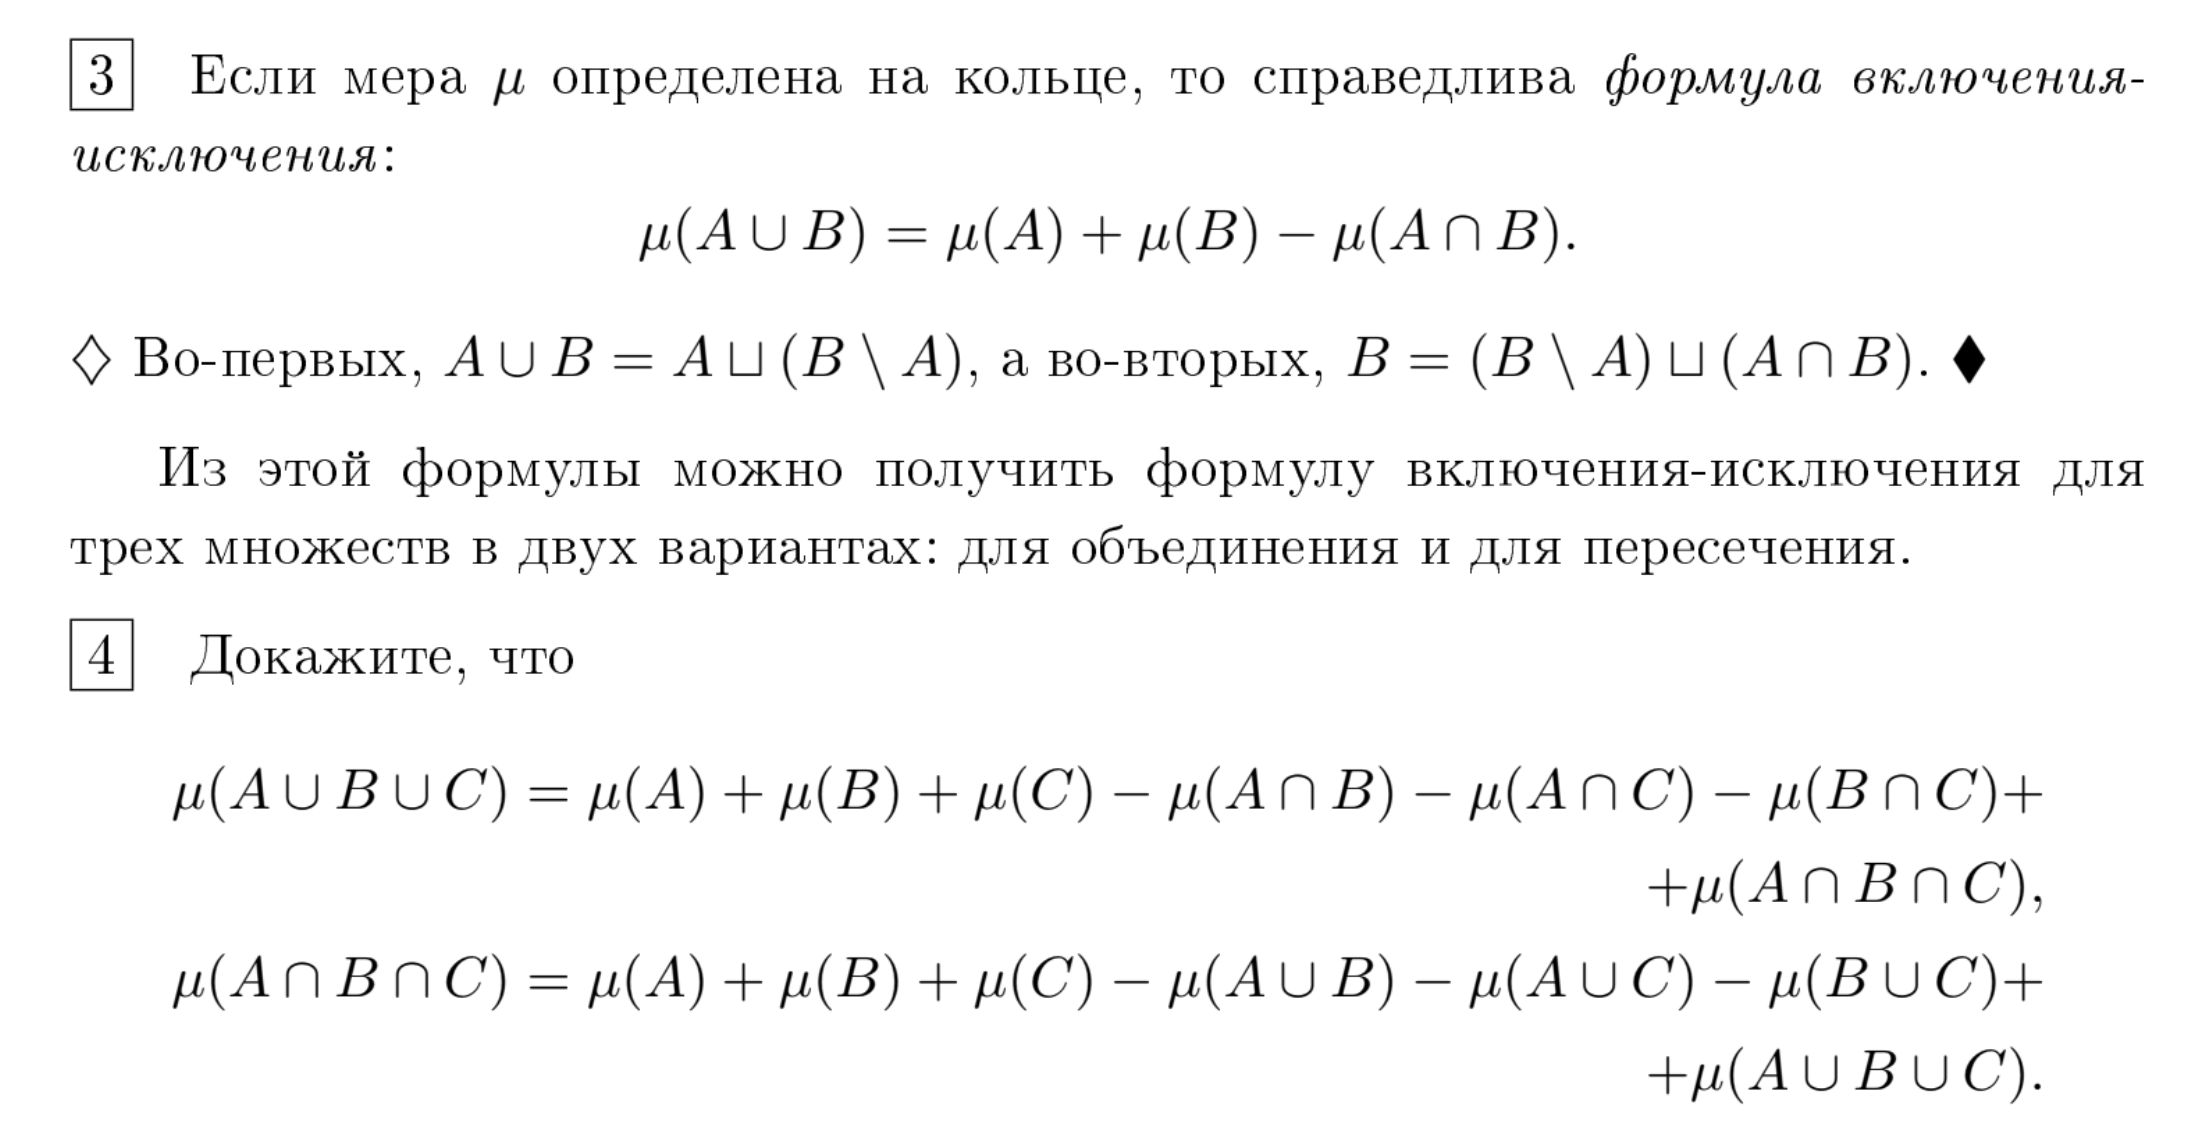
\includegraphics[scale=0.3]{1.png}
\end{center}
Будем идти аналогично док-ву для двух множеств и использовать определение $\mu(A \sqcup B) = \mu(A) + \mu(B)$, посмотрим на объединение и воспользуемся формулой включений-исключений для двух множеств:
\[
\mu(A \; \cup \; B \; \cup \; C) = \mu ((A \; \cup \;B) \;\sqcup \; \left[C\; \backslash \; (A \; \cup \;  B)\right]) = \mu(A \; \cup \;  B) + \mu (C \backslash (A \; \cup \; B)) = 
\]
\begin{equation*}
\begin{gathered}
= \mu(A) + \mu(B) - \mu(A \cap B)+ \mu (C\; \backslash\; (A \; \cup \; B)) =
\end{gathered}
\end{equation*}
На семинаре делали $\mu(A \backslash B)$
\begin{equation*}
\begin{gathered}
=
\mu(A) + \mu(B) - \mu(A \cap B) + \mu(C) - \mu(C \cap (A \cup B)) =
\\
=
 \mu(A) + \mu(B) - \mu(A \cap B) + \mu(C) - \mu((C \cap A) \cup (C \cap B))
\end{gathered}
\end{equation*}
Раскроем $\mu((C \cap A) \cup (C \cap B))$ как формулу включений-исключений:
\begin{equation*}
\begin{gathered}
\mu((C \cap A) \cup (C \cap B)) = \mu(C \cap A) + \mu(C \cap B) - \mu(C \cap A \cap C \cap B) =
\\
=
 \mu(A \cap C) + \mu(C \cap B) -  \mu(A \cap B \cap C)
\end{gathered}
\end{equation*}
Возвращаемся к исходной формуле:
\begin{equation*}
\begin{gathered}
\mu(A  \cup  B \cup C) = \mu(A) + \mu(B) - \mu(A \cap B) + \mu(C) - \mu(A \cap C) - \mu(C \cap B) + \mu(A \cap B \cap C) =
\\
=
\mu(A) + \mu(B) + \mu(C) - \mu(A \cap B) - \mu(A \cap C) - \mu(B \cap C) + \mu(A \cap B \cap C)
\end{gathered}
\end{equation*}
Получили то, что хотели, теперь выразим пересечения (перенесем на другую сторону:):
\begin{equation*}
\begin{gathered}
\mu(A \cap B \cap C) = \mu(A \cup B \cup C) - \mu(A) - \mu(B) - \mu(C)  + \mu(A \cap B) + \mu(A \cap C) + \mu(B \cap C)
\end{gathered}
\end{equation*}
Теперь можем представить формулу в том виде, который присутствует в конспекте под пунктом 4 (не знаю зачем, но пусть будет), из формулы включений-исключений для 2 элементов знаем:
\begin{equation*}
\begin{gathered}
\mu(A \cap B) = \mu(A) + \mu(B) - \mu(A \cup B)
\end{gathered}
\end{equation*}
Тогда:
\begin{equation*}
\begin{gathered}
\mu(A \cap B \cap C) = \mu(A \cup B \cup C) - \mu(A) - \mu(B) - \mu(C)  + \mu(A) + \mu(B) -
\\
-
 \mu(A \cup B) + \mu(A) + \mu(C) - \mu(A \cup C) + \mu(B) + \mu(C) - \mu(B \cup C) = 
\\
=
\mu(A) + \mu(B) + \mu(C) - \mu(A \cup B) - \mu(A \cup C) - \mu(B \cup C) + \mu(A \cup B \cup C)
\end{gathered}
\end{equation*}
\begin{center}
\textbf{Ответ: } \begin{equation*}
\begin{gathered}
\mu(A \cap B \cap C) = \mu(A) + \mu(B) + \mu(C) - \mu(A \cup B) - \mu(A \cup C) - \mu(B \cup C) + \mu(A \cup B \cup C)
\end{gathered}
\end{equation*}
\end{center}
\clearpage
\section*{Номер 2}
Пусть:
\[
A_1, A_2 - \text{ измеримы}
\]
\[
E_1 \supseteq A_1
\]
\[
E_2 \supseteq A_2
\]
\[
A_1 \cap A_2 \subseteq E_1 \cap E_2
\]
Тогда:
\[
(E_1 \cap E_2)\;  \backslash \; (A_1 \cap A_2) \subseteq (E_1 \backslash A_1) \cup (E_2 \backslash A_2) 
\]
Пусть:
\[
E_1 \cap E_2 = E
\]
\[
A_1 \cap A_2 = A
\]
Получаем:
\[
\overline{\mu} (E\; \backslash\; A) \leq \overline{\mu}\left((E_1 \backslash A_1) \cup (E_2 \backslash A_2) \right) \leq \overline{\mu} (E_1 \backslash A_1) +  \overline{\mu} (E_2 \backslash A_2) 
\]
Знаем из условия, что $A_1$ и $A_2$ измеримы, тогда можем положить:
\[
 \overline{\mu} (E_1 \backslash A_1)  < \frac{\varepsilon}{2}
\]
\[
\overline{\mu} (E_2 \backslash A_2)  < \frac{\varepsilon}{2}
\]
Итого:
\[
\overline{\mu} (E\; \backslash\; A)  < \frac{\varepsilon}{2} + \frac{\varepsilon}{2} = \varepsilon
\]
Смогли предоставить $\varepsilon$, тогда по определению множество $A_1 \cap A_2$ является измеримым множеством
\begin{center}
\textbf{Ч.Т.Д} 
\end{center}
\end{document}
